\chapter{The CMS Experiment at the Large Hadron Collider}\label{chap:cms}
The data used in this analysis is from $pp$ collisions produced by the Large Hadron Collider (LHC) and was recorded using the Compact Muon Solenoid (CMS) detector during the years 2016-2018. In this chapter, I will briefly explain the LHC complex and describe the CMS detector in detail, focusing on the subdetectors relevant to this analysis (the tracker and calorimeters).
\section{The Large Hadron Collider}
The Large Hadron Collider is the world's largest particle accelerator used for the study of proton-proton ($pp$) and heavy-ion (HIN) collisions. It is located outside of Geneva, Switzerland and its operation is overseen by the European Organization for Nuclear Research (Conseil Européen pour la Recherche Nucléaire - CERN). The LHC occupies a 26.7 km in circumference tunnel that originally housed the Large Electron-Positron (LEP) collider \cite{LEP}, and lies between 45m and 170m underground. The LHC was designed to deliver $pp$ collisions at a center of mass energy $\sqrt{s} = \sqrt{4E_{p_1}E_{p_2}}=14$ TeV and instantaneous luminosity of $\mathcal{L} = 10^{34}\mathrm{cm}^2\mathrm{s}^{-1}$ and to collide Pb ions at 2.76 GeV/nucleon at $\mathcal{L}=20^{27}\mathrm{cm}^2\mathrm{s}^-1$ and was constructed between 1998 and 2008.\\
Although we normally describe the LHC as a circular collider, it actually contains 528m long eight straight sections where the experiments and beam facilties are housed between arcs where the protons or ions are trajectories are bent.
\begin{figure}
    \centering
    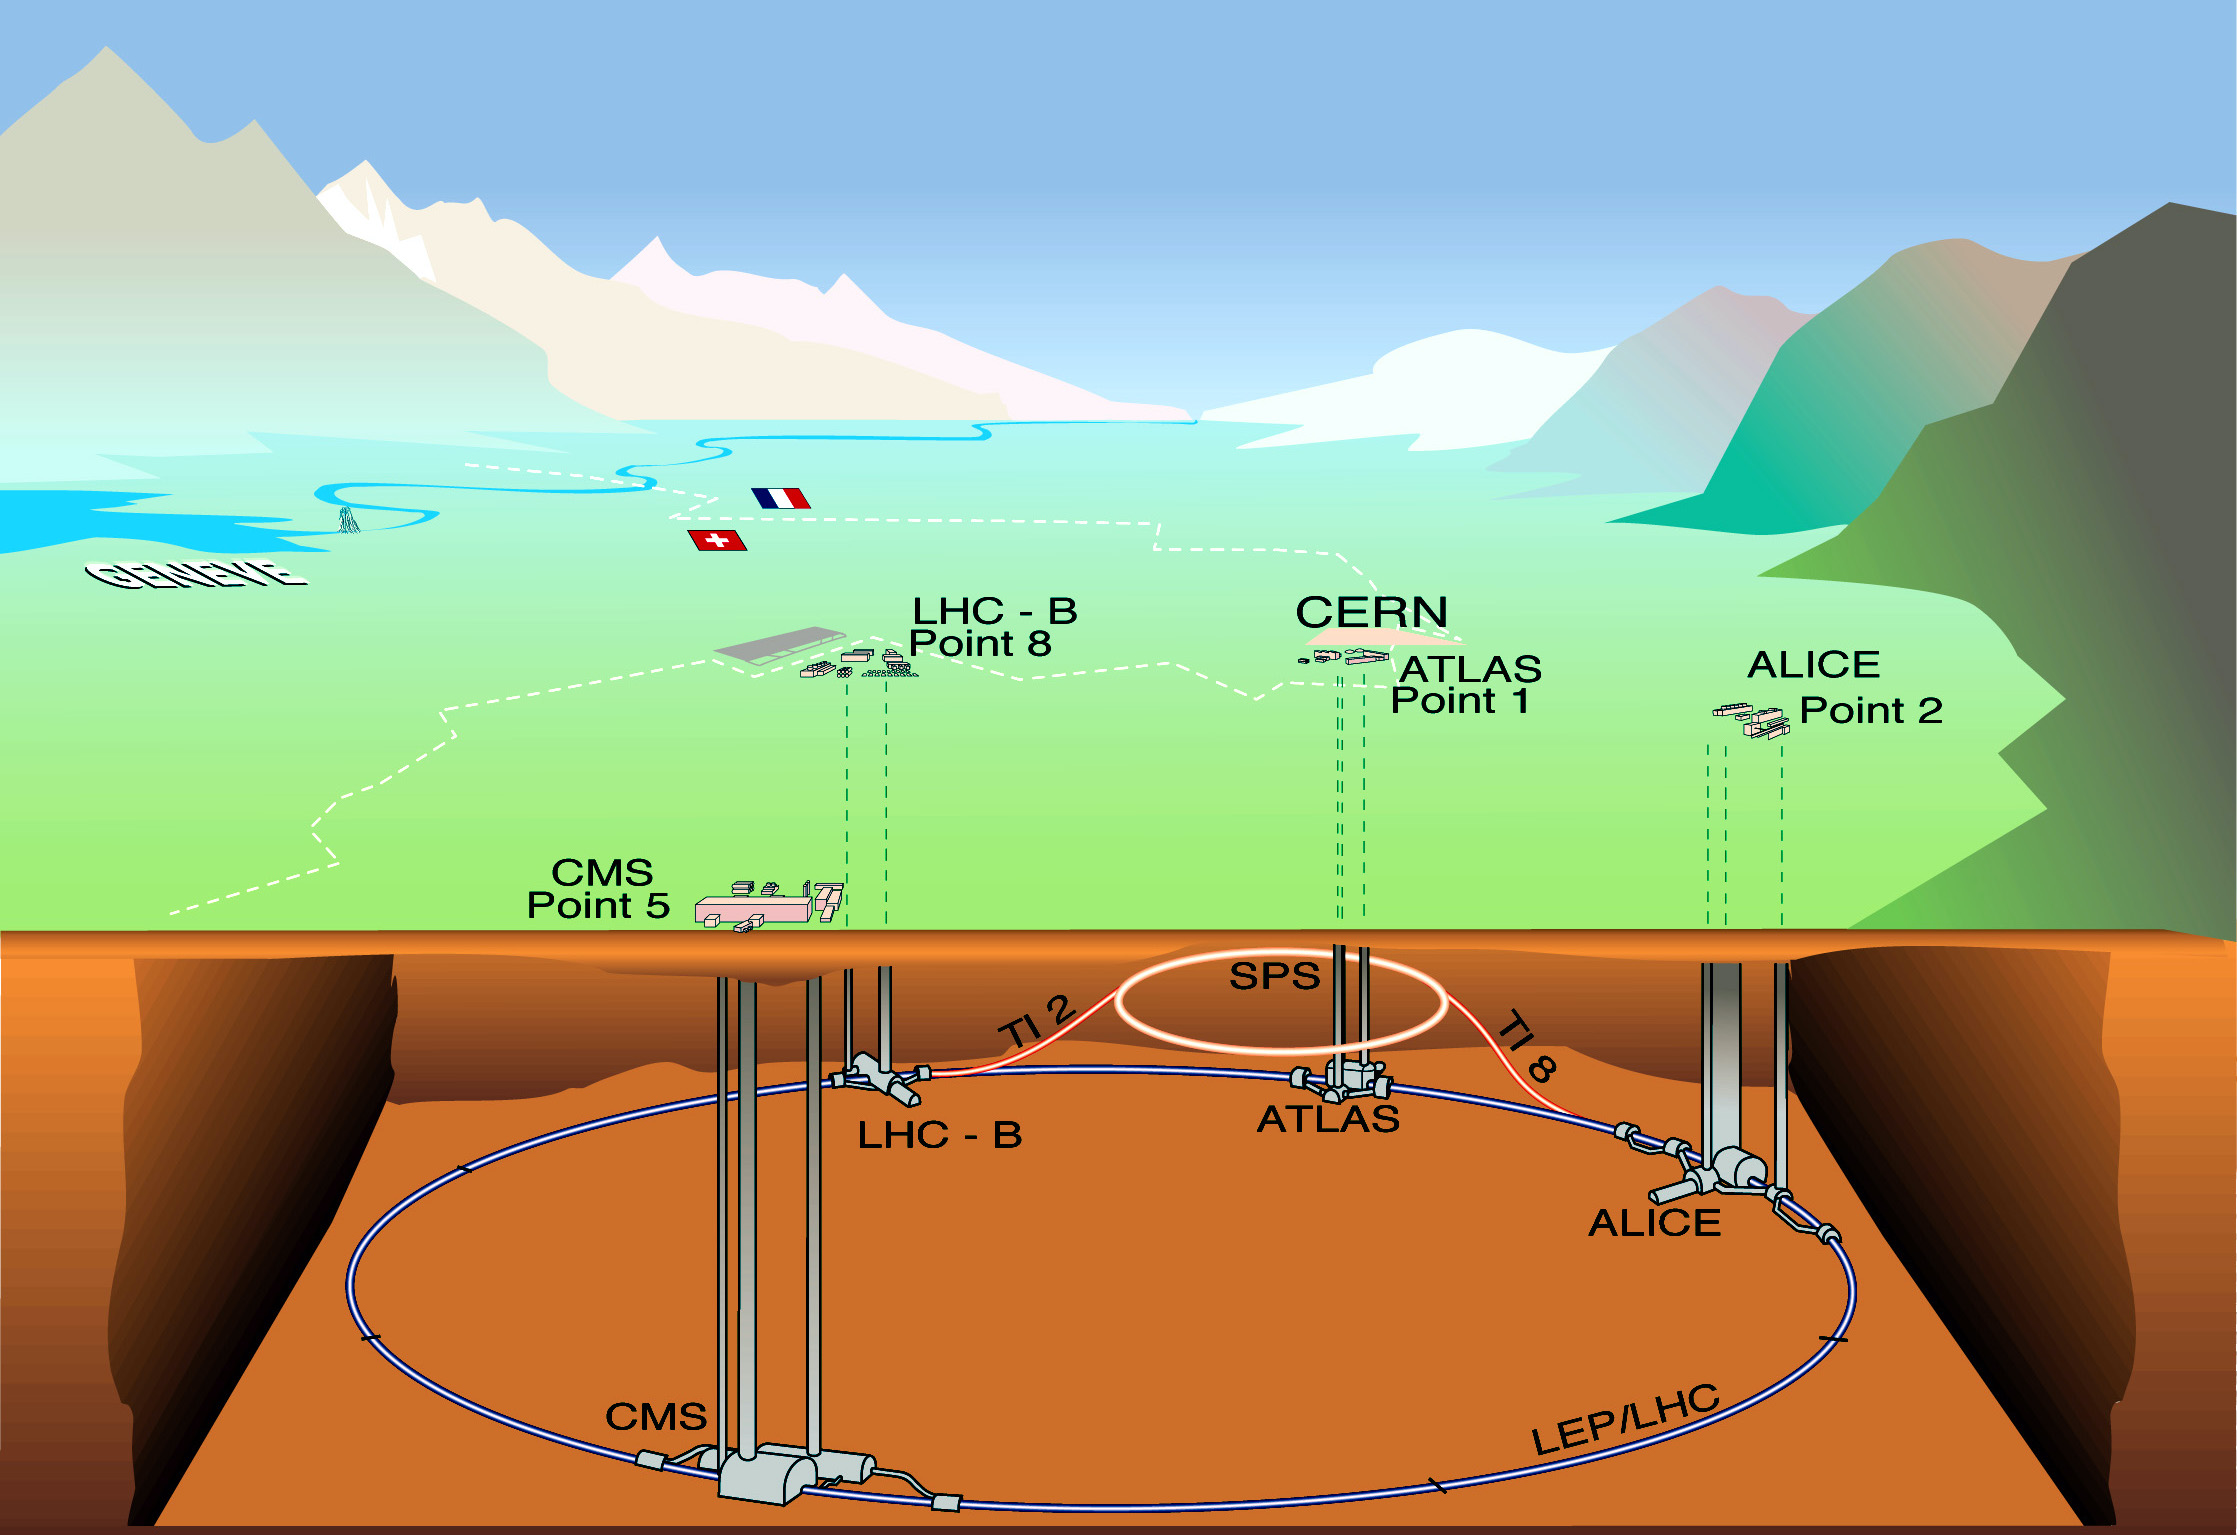
\includegraphics[width=\linewidth]{figures/LHC-PHO-1997-237.jpg}
    \caption{Schematic of the Large Hadron Collider showing its location along the French-Swiss border and where the four main detectors are located along its ring \cite{LHCMap}. }
    \label{fig:LHCmap}
\end{figure}



\section{The Compact Muon Solenoid}